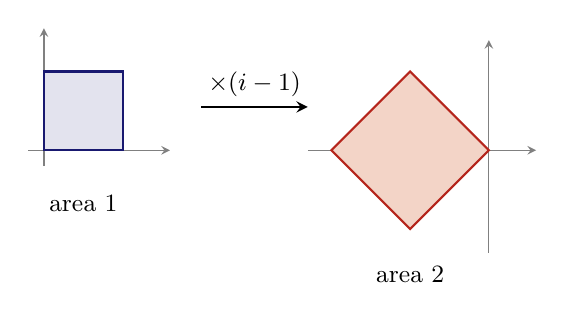
\begin{tikzpicture}[x=1cm,y=1cm,font=\small,>=stealth]
\begin{scope}
\draw[gray,->] (-.2,0)--(1.6,0);
\draw[gray,->] (0,-.2)--(0,1.55);
\fill[MidnightBlue!12] (0,0)--(1,0)--(1,1)--(0,1)--cycle;
\draw[MidnightBlue,thick] (0,0)--(1,0)--(1,1)--(0,1)--cycle;
\node[below] at (.5,-.45) {area $1$};
\end{scope}
\draw[->,thick] (2,.55)--node[above] {$\times(i-1)$} (3.35,.55);
\begin{scope}[shift={(5.65,0)}]
\draw[gray,->] (-2.3,0)--(.6,0);
\draw[gray,->] (0,-1.3)--(0,1.4);
\fill[BrickRed!15] (0,0)--(-1,1)--(-2,0)--(-1,-1)--cycle;
\draw[BrickRed,thick] (0,0)--(-1,1)--(-2,0)--(-1,-1)--cycle;
\node[below] at (-1,-1.35) {area $2$};
\end{scope}
\end{tikzpicture}
